\section{Bundle Adjustment}
\label{sec:bundle}

Bundle Adjustment is commonly used as the last step of every feature-based 3D reconstruction algorithm. Given a set of images depicting a number of 3D points from different viewpoints, bundle adjustment is the process of simultaneously refining the 3D coordinates along with the camera parameters. It minimizes reprojection error, which is the squared sum of distances between image points and predicted points. In this section, you will implement bundle adjustment algorithm by yourself (make use of \texttt{q5\_bundle\_adjustment.py} file). Specifically,

\begin{itemize}
    \item In Q5.1, you need to implement a RANSAC algorithm to estimate the fundamental matrix $\F$ and all the inliers.
    
    \item In Q5.2, you will need to write code to parameterize Rotation matrix $\mathbf{R}$ using  \href{https://en.wikipedia.org/wiki/Rodrigues\%27\_formula}{\textcolor{blue}{Rodrigues formula}} (please check \href{https://www2.cs.duke.edu/courses/fall13/compsci527/notes/rodrigues.pdf}{\textcolor{blue}{this pdf}} for a detailed explanation), which will enable the joint optimization process for Bundle Adjustment.
    
    \item In Q5.3, you will need to first write down the objective function in \texttt{rodriguesResidual}, and do the \texttt{bundleAdjustment}.
\end{itemize}

\subparagraph*{Q5.1 RANSAC for Fundamental Matrix Recovery}\points{15}
In some real world applications, manually determining correspondences is infeasible and often there will be noisy correspondences. Fortunately, the RANSAC method seen in class can be applied to the problem of fundamental matrix estimation.

Implement the above algorithm with the signature:
\begin{center}
\texttt{[F, inliers] = ransacF(pts1, pts2, M, nIters, tol)}
\end{center}
where \texttt{M} is defined in the same way as in \autoref{sec:fundmatrix} and inliers is a boolean vector of size equivalent to the number of points. Here inliers is set to true only for the points that satisfy the threshold defined for the given fundamental matrix $\F$.

We have provided some noisy correspondences in \texttt{some\_corresp\_noisy.npz} in which around $75\%$ of the points are inliers. 

\deliver{
\textbf{In your write-up:} Compare the result of RANSAC with the result of the eightpoint when ran on the noisy correspondences. Briefly explain the error metrics you used, how you decided which points were inliers, and any other optimizations you may have made. \texttt{nIters} is the maximum number of iterations of RANSAC and \texttt{tol} is the tolerance of the error to be considered as inliers. Discuss the effect on the Fundamental matrix by varying these values. \textbf{Please include the code snippet of the \texttt{ransacF} function in your write-up.}
}

\begin{itemize}
    \item \emph{Hints:} Use the Eight or Seven point algorithm to compute the fundamental matrix from the minimal set of points. Then compute the inliers, and refine your estimate using all the inliers.
\end{itemize}

\begin{your_solution}[title=Q5.1,height=5.5cm,width=\linewidth]
\end{your_solution}

\subparagraph*{Q5.2 Rodrigues and Invsere Rodrigues}\points{15}
So far we have independently solved for camera matrix, $\mathbf{M}_j$ and 3D points $\w_i$. In bundle adjustment, we will jointly optimize the reprojection error with respect to the points $\w_i$ and the camera matrix $\C_j$.
$$
err = \sum_{ij} \|\x_{ij} - Proj(\mathbf{C}_j, \w_i)\|^2,
$$
where $\C_j = \mathbf{K}_j \mathbf{M}_j$, same as in Q3.2.

For this homework we are going to only look at optimizing the extrinsic matrix. To do this we will be parameterizing the rotation matrix $\mathbf{R}$ using Rodrigues formula to produce vector $\mathbf{r} \in \mathbb{R}^3$. Write a function that converts a Rodrigues vector $\mathbf{r}$ to a rotation matrix $\mathbf{R}$
\begin{center}
\texttt{R = rodrigues(r)}
\end{center}
as well as the inverse function that converts a rotation matrix $\mathbf{R}$ to a Rodrigues vector~$\mathbf{r}$
\begin{center}
\texttt{r = invRodrigues(R)}
\end{center}
Reference: \href{https://en.wikipedia.org/wiki/Rodrigues\%27\_formula}{\textcolor{blue}{Rodrigues formula}} and \href{https://www2.cs.duke.edu/courses/fall13/compsci527/notes/rodrigues.pdf}{\textcolor{blue}{this pdf}}.

\deliver{
\textbf{In your write-up:} Include the code snippet of \texttt{rodrigues} and \texttt{invRodrigues} functions.
}

\begin{your_solution}[title=Q5.2,height=5.5cm,width=\linewidth]
\end{your_solution}

\subparagraph*{Q5.3 Bundle Adjustment}\points{10}

Using this parameterization, write an optimization function
\begin{center}
\texttt{residuals = rodriguesResidual(K1, M1, p1, K2, p2, x)}
\end{center}
where \texttt{x} is the flattened concatenation of $\mathbf{x}$, $\mathbf{r}_2$, and $\mathbf{t}_2$. $\mathbf{w}$ are the 3D points; $\mathbf{r}_2$ and $\mathbf{t}_2$ are the rotation (in the Rodrigues vector form) and translation vectors associated with the projection matrix $\mathbf{M}_2$. The \texttt{residuals} are the difference between original image projections and estimated projections (the square of $L2$-norm of this vector corresponds to the error we computed in Q3.2):
\begin{center}
\texttt{residuals = numpy.concatenate([(p1-p1\_hat).reshape([-1]), (p2-p2\_hat).reshape([-1])])}
\end{center}

Use this error function and Scipy's optimizer $\texttt{minimize}$ to write a function that optimizes for the best extrinsic matrix and 3D points using the inlier correspondences from \texttt{some\_corresp\_noisy.npz} and the RANSAC estimate of the extrinsics and 3D points as an initialization.

\begin{center}
\texttt{[M2, w, o1, o2] = bundleAdjustment(K1, M1, p1, K2, M2\_init, p2, w\_init)}
\end{center}

Try to extract the rotation and translation from \texttt{M2\_init}, then use \texttt{invRodrigues} you implemented previously to transform the rotation, concatenate it with translation and the 3D points, then the concatenate vector are variables to be optimized. After obtaining optimized vector, decompose it back to rotation using \texttt{rodrigues} you implemented previously, translation and 3D points coordinates.

\deliver{
\textbf{In your write-up}: 
\begin{itemize}
    \item Include an image of the original 3D points and the optimized points (use the provided \texttt{plot\_3D\_dual} function).
    \item Report the reprojection error with your initial $\mathbf{M}_2$ and $\mathbf{w}$, as well as with the optimized matrices. 
    \item Include the code snippets for \texttt{rodriguesResidual} and \texttt{bundleAdjustment} in your write-up.
\end{itemize}
}

\textit{Hint:} For reference, our solution achieves a reprojection error around 10 after optimization. Your exact error may differ slightly. 

\begin{your_solution}[title=Q5.3,height=5.5cm,width=\linewidth]
\end{your_solution}

\begin{figure}[h!]
    \centering
    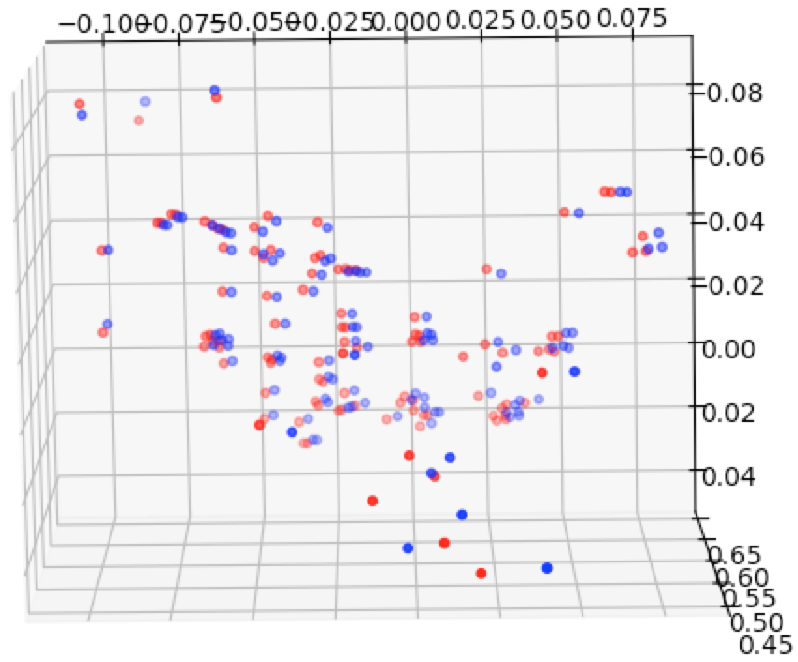
\includegraphics[width=0.45\textwidth]{images/q5_3.png}
    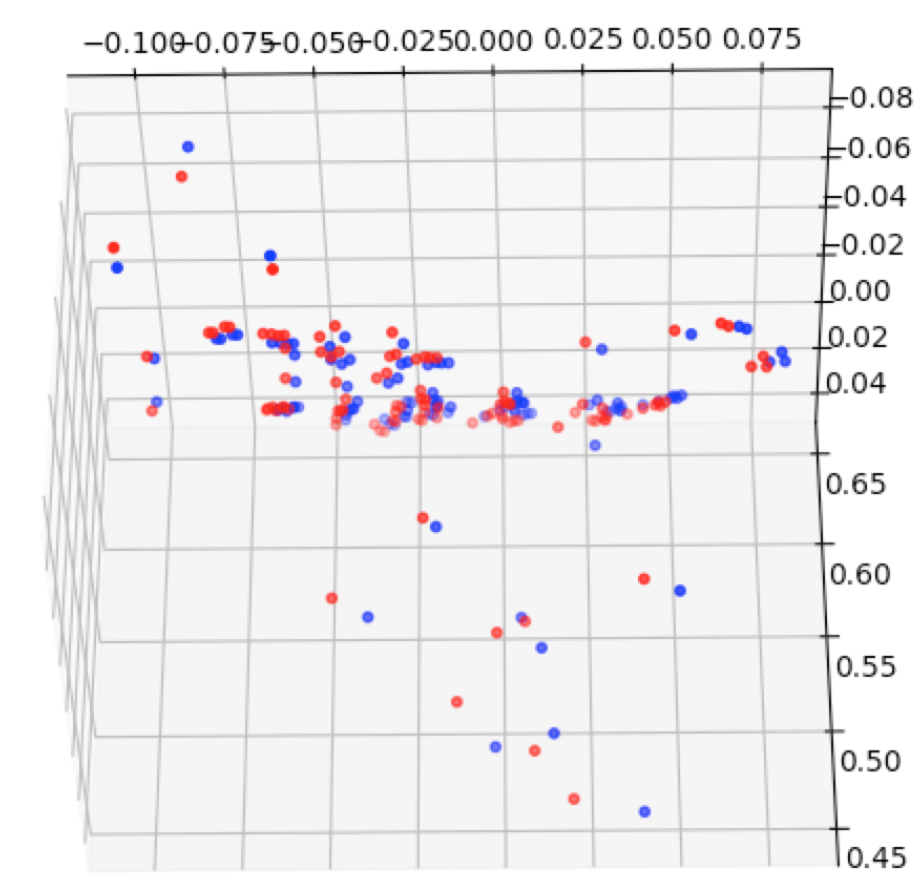
\includegraphics[width=0.4\textwidth]{images/q5_3b.png}
\caption{Visualization of 3D points for noisy correspondences before and after using bundle
adjustment}
    \label{fig:q5}
\end{figure}